\documentclass{sigchi-ext}
% Please be sure that you have the dependencies (i.e., additional
% LaTeX packages) to compile this example.
\usepackage[T1]{fontenc}
\usepackage{textcomp}
\usepackage[scaled=.92]{helvet} % for proper fonts
\usepackage{graphicx} % for EPS use the graphics package instead
\usepackage{balance}  % for useful for balancing the last columns
\usepackage{booktabs} % for pretty table rules
\usepackage{ccicons}  % for Creative Commons citation icons
\usepackage{ragged2e} % for tighter hyphenation

% Some optional stuff you might like/need.
% \usepackage{marginnote} 
% \usepackage[shortlabels]{enumitem}
% \usepackage{paralist}
\usepackage[utf8]{inputenc} % for a UTF8 editor only

%% EXAMPLE BEGIN -- HOW TO OVERRIDE THE DEFAULT COPYRIGHT STRIP --
% \copyrightinfo{Permission to make digital or hard copies of all or
% part of this work for personal or classroom use is granted without
% fee provided that copies are not made or distributed for profit or
% commercial advantage and that copies bear this notice and the full
% citation on the first page. Copyrights for components of this work
% owned by others than ACM must be honored. Abstracting with credit is
% permitted. To copy otherwise, or republish, to post on servers or to
% redistribute to lists, requires prior specific permission and/or a
% fee. Request permissions from permissions@acm.org.\\
% {\emph{CHI'14}}, April 26--May 1, 2014, Toronto, Canada. \\
% Copyright \copyright~2014 ACM ISBN/14/04...\$15.00. \\
% DOI string from ACM form confirmation}
%% EXAMPLE END

% Paper metadata (use plain text, for PDF inclusion and later
% re-using, if desired).  Use \emtpyauthor when submitting for review
% so you remain anonymous.
\def\plaintitle{SIGCHI Extended Abstracts Sample File: Note Initial
  Caps} \def\plainauthor{First Author, Second Author, Third Author,
  Fourth Author, Fifth Author, Sixth Author}
\def\emptyauthor{}
\def\plainkeywords{Authors' choice; of terms; separated; by
  semicolons; include commas, within terms only; required.}
\def\plaingeneralterms{Documentation, Standardization}

\title{Erstellung, Suche und Vergleich von Phantombildern in der Augmented Reality}

\numberofauthors{3}
% Notice how author names are alternately typesetted to appear ordered
% in 2-column format; i.e., the first 4 autors on the first column and
% the other 4 auhors on the second column. Actually, it's up to you to
% strictly adhere to this author notation.
\author{%
  \alignauthor{%
    \textbf{Alexandra Krien}\\ 
    \affaddr{Interactive Media Lab} \\
    \affaddr{Technische Universität Dresden} \\
    \affaddr{Dresden, Germany} \\
    \email{alexandra.krien@tu-dresden.de} } \vfil \alignauthor{%
    \textbf{Maxime Thebault}\\
    \affaddr{VP, Authoring}\\
    \affaddr{Authorship Holdings, Ltd.}\\
    \affaddr{Awdur SA22 8PP, UK}\\
    \email{Maxime.Thebault@insa-rennes.fr} } \vfil \alignauthor{%
    \textbf{Heiner Ludwig}\\
   \affaddr{Interactive Media Lab} \\
    \affaddr{Technische Universität Dresden} \\
    \affaddr{Dresden, Germany} \\
    \email{heiner.ludwig@tu-dresden.de} }}

% Make sure hyperref comes last of your loaded packages, to give it a
% fighting chance of not being over-written, since its job is to
% redefine many LaTeX commands.
\definecolor{linkColor}{RGB}{6,125,233}
\hypersetup{%
  pdftitle={\plaintitle},
%  pdfauthor={\plainauthor},
  pdfauthor={\emptyauthor},
  pdfkeywords={\plainkeywords},
  bookmarksnumbered,
  pdfstartview={FitH},
  colorlinks,
  citecolor=black,
  filecolor=black,
  linkcolor=black,
  urlcolor=linkColor,
  breaklinks=true,
}

% \reversemarginpar%

\begin{document}

%% For the camera ready, use the commands provided by the ACM in the Permission Release Form.
%\CopyrightYear{2016}
%\setcopyright{rightsretained}
%\conferenceinfo{WOODSTOCK}{'97 El Paso, Texas USA}
%\isbn{0-12345-67-8/90/01}
%\doi{http://dx.doi.org/10.1145/2858036.2858119}
%% Then override the default copyright message with the \acmcopyright command.
%\copyrightinfo{\acmcopyright}

\maketitle

% Uncomment to disable hyphenation (not recommended)
% https://twitter.com/anjirokhan/status/546046683331973120
\RaggedRight{} 

% Do not change the page size or page settings.
\begin{abstract}
  Phantombilder sind in der Polizeiarbeit ein unverzichtbares Medium bei der Suche nach Verdächtigen. Diese Arbeit beschäftigt sich damit, wie die dabei gängigen Abläufe in die Augmented Reality angehoben werden können um so die Bedienbarkeit und Nutzererfahrung zu verbessern. Fokus liegt dabei auf einer anfragebasierten, unscharfen Suche anhand der Phantombilder auf einer Datenbank von standardisierten Fotografien verschiedener Personen. Der Nutzer hat so die Möglichkeit seine zusammengestellten (Such-)Kriterien anhand reeller Menschen zu vergleichen und möglicherweise seine Anfrage auf der Suche nach dem besten Treffer anzupassen.
\end{abstract}

\keywords{Information Retrieval, Phantombilder, Augmented Reality}

\section{Einführung}
 Auf der Suche nach bestimmten Personen, beispielsweise im Zuge der Ermittlung einer Straftat, sind Phantombilder ein gängiges Hilfsmittel. Augenzeugen versuchen ihre Erinnerung unter Anleitung eines Beamten zu rekonstruieren. Auch wenn die Erstellung solcher Phantombilder bereits auf eine digitale Ebene angehoben wurde, ist der Prozess dennoch bisher sehr statisch. Die skizzenhaft zusammengestellten Merkmale enthalten möglicherweise große Ungenauigkeiten, Nutzer haben keine Möglichkeit ihr Ergebnis mit reellen Menschen abzugleichen. Hinzu kommt der große Einfluss eines anwesenden Beamten. Der Zeuge muss seine Erinnerungen sehr genau und eindeutig beschreiben, um auf der gleichen Ebene dessen zu kommunizieren, da beispielsweise die Beschreibung einer "'hellen Haut"' unterschiedlich aufgefasst werden kann.
 
Die Idee hinter dieser Arbeit ist es Phantombilder als Anfrage für ein datenbankbasiertes System zu nutzen. Dies bietet die Möglichkeit die skizzenhafte Anfrage mit reellen Menschen zu vergleichen. Personen fallen so möglicherweise eher Fehler oder Ungenauigkeiten auf und haben die Möglichkeit ihre Anfrage iterativ so weit zu verfeinern, dass die Ergebnismenge der verdächtigen Personen eher ihrer Erinnerung entspricht. Diese Menge ist eineindeutig.

Ziel soll ein intuitives System sein, welches nach einer Einführung selbstständig von Personen ohne Vorwissen eingesetzt werden kann. Um dem Nutzer einen persönlichen Bearbeitungsraum zu bieten und an die reelle Begegnung anzuknüpfen, wurde entschieden dieses System in die Augmented Reality anzuheben. Gesten sollen dabei als einfache Interaktionsform dienen.

\section{Verwandte Arbeiten}
\subsubsection{Erstellung von Phantombildern}
Die klassische Erstellung von Phantombildern findet im Rahmen einer Zeugenaussage auf dem Revier statt. Die Umgebung kann dabei Auswirkungen auf die Genauigkeit der Aussage haben. Erfahrungen zeigten, dass insbesondere anwesende Beamte Einfluss auf die Ergebnisse nahmen. Ihre Aufgabe ist es die Zeugen bei der Rekonstruktion des Gesehenen zu unterstützen. Soziale Faktoren entscheiden dabei darüber wie viele Informationen tatsächlich preisgegeben und ob sie korrekt aufgenommen werden. So können unterschiedliche Vorstellungen und Auffassungen zur Ausprägung von Merkmalen zu Abweichungen führen. Alle beteiligten Personen müssen demnach für ein gutes Ergebnis die gleiche deskriptive Sprache sprechen. ~\cite{buchholz:stimme}

Dieser klassische Prozess wurde bereits in der Vergangenheit versucht auf eine digitale Ebene anzuheben. So existieren eine Vielzahl an einfachen Desktoplösungen, die ein Zusammenstellen verschiedener optischer Merkmale zu einem Phantombild erlauben.
Die konkrete Suche aufgrund eines veränderbaren Phantombildes hingegen ist unseren Recherchen zu Folge noch nicht so verbreitet. Die wenigen existierenden Systeme brachten aber bereits Erkenntnisse darüber, wie ein moderner Erstellungsprozess ablaufen könnte und welche Faktoren entscheidend sind, um durch die Anfrage auch signifikante Ergebnisse zu erhalten.

Unterschiede zeigten sich insbesondere durch die Auswahl der kombinierbaren Merkmale für die Suchanfrage. "'SpotIt!"' beispielsweise ermöglicht die Auswahl mehrerer Ausprägungen für ein Merkmal und interpoliert anschließend zwischen diesen um die optimale Lösung zu finden. ~\cite{brunelli1996} Ein anderes Personenidentifikationssystem hingegen zeigte, dass bereits eine Unterscheidung des Gesichts in 3 Bereiche reicht, um in der Suche eine Trefferquote von über 90\% zu erreichen. Wichtigster Faktor ist dabei die Ausprägung der Augen. ~\cite{bobulski2012}

\subsubsection{Gesten}
Gestik als Eingabemedium zur Erstellung von Phantombildern ist gänzlich neu, der Aufbau einer geeigneten Gesten-Sprache demnach unumgänglich. 

Das Buch Emotionales Interaktionsdesign beschäftigt sich
 u.a. mit der Semantik von Gestensprachen und zeigt Notwendigkeiten wie Abbruch-Gesten oder die allgemeine Robustheit von Gesten auf~\cite{Dorau11}. Kaisa Väänänen und Klaus Böhm weisen auf Schwierigkeiten wie Ermüdung der Gliedma{\ss}en und eingeschränkte Exaktheit während der Gesten-Nutzung hin, betonen jedoch gleichzeitig die vereinfachte Navigation und Manipulation für verschiedenste Nutzergruppen in virtuellen 3D-Räumen~\cite{vrs:book}.
In~\cite{3dinteraction:book} ist laut einer Nutzerstudie die
Metaphern-Nutzung bei Gesten weniger effektiv als die Nutzung von
Freihand-Gesten. 

Gemä{\ss} [7,8] ist allgemein die Nutzung von formalisierten Gesten (``semaphoric gestures'') nicht sinnvoll, da sie während der Interaktion unnatürlich wirkt.
~\cite{3dinteraction:book} besagt jedoch, dass beim Gro{\ss}teil der
gestenbasierten Eingabesysteme sowohl formalisierte, als auch
Freihand-Gesten genutzt werden.

Nicht zuletzt haben Hollywood-Filme wie \textit{Iron Man}~\cite{ironman:movie} oder \textit{Minority Report}~\cite{minorityreport:movie} zur Inspiration für die User Experience und bei der Erstellung der Nutzungsoberfläche gedient.

Zur Kombination von Virtueller Realität mit Gestenmanipulation haben die Firmen \textit{eyeSight\footnote{\url{eyesight-tech.com/vr-ar.html}}} und 
\textit{pebbles\footnote{\url{www3.oculus.com/en-us/blog/pebbles-interfaces-joins-oculus/}}} unabhängig voneinander eine VR-Brille mit mehreren Kameras kombiniert um die Interaktion mit dem virtuellen Raum für den Nutzer möglich zum machen.

\begin{figure}
  \centering
  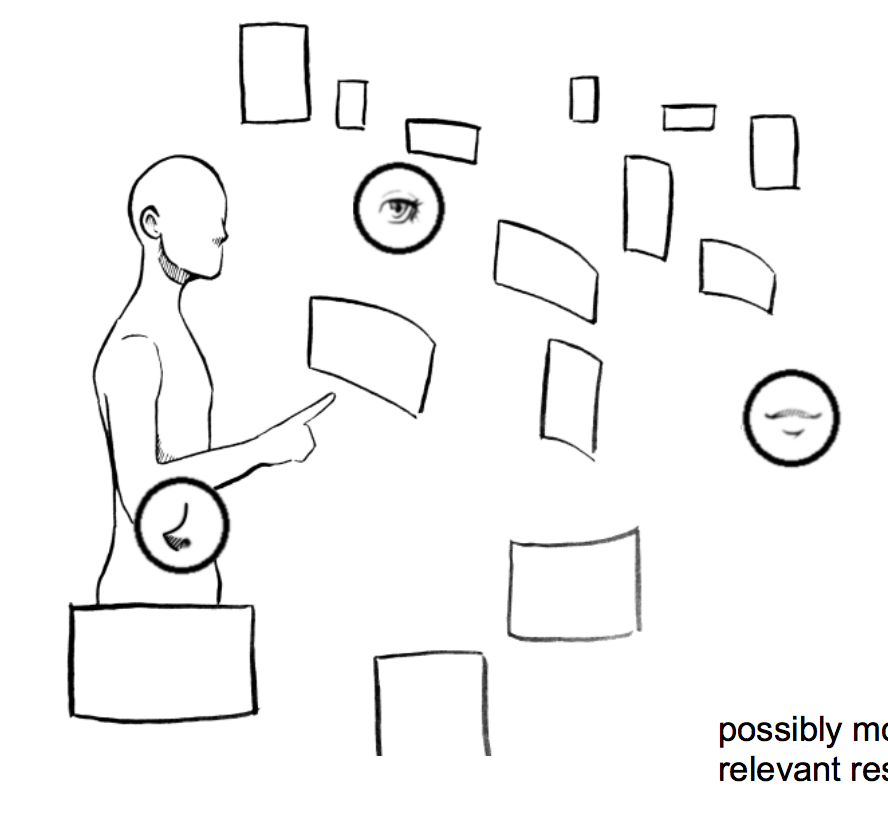
\includegraphics[width=1\marginparwidth]{figures/system_overview}
  \caption{Virtuelle Objekte im System}
  \label{fig:systemoverview}
\end{figure}

\section{Konzept}

Das Konzept zur digitalen Erstellung von Phantombildern ist ein digitales System, welches den Nutzer in eine virtuelle Realität versetzt, die mittels Gesten manipulierbar ist. Durch die Interaktion mit suchanfragen- und ergebnisrepräsentierenden Objekten steuert der Nutzer die Erstellung des Phantombildes, indem er diese Objekte auswählt, verschiebt, löscht oder kombiniert. 

Der Nutzer navigiert das System von einem Punkt aus. Um einzelne Objekte genauer zu betrachten, bewegt er sich also nicht körperlich, sondern verändert die Position des virtuellen Raums mittels Translations- und Skalierungsgesten.

Die Objekte sind im 180-Winkel "schwebend" um den Nutzer angeordnet (Figure~\ref{fig:systemoverview}). Durch sowohl freie, als auch objektorientierte Gesten, kann er, mittels ein- oder zweihändiger Gestikulation, Suchanfragen, Ergebnisse oder Ergebnisvorschläge speichern, löschen, zum Ergebnis-pool hinzufügen, neu kombinieren oder rückgängig machen.
Das System wird immer nur von einem Nutzer gleichzeitig benutzt,
weitere Personen können während des gesamten Findungsprozesses
ausschließlich als Zuschauer involviert werden. So ist eine
Moderatorenrolle eines Experten denkbar, der Hilfestellung gibt.

Aus der Sicht der Nutzbarkeit bietet das System folgende Vorteile:
\begin{itemize}\compresslist%
\item Effizientes und selbstständiges Arbeiten durch intuitive Gesten und Hilfestellung durch das System.
\item Sehr direkte Interaktion vom Nutzer mit der Benutzungsoberfläche.
\item Effektive Ergebnisfindung durch ständiges Feedback und Anpassung vom System.
\item Nutzerbefriedigung durch immer sichtbaren Fortschritt.
\item Einsatz ist ortsunabhängig und verlangt nur kleine Räumlichkeiten
\end{itemize}

\section{Systemnutzung}
\subsubsection{Systemstart und erste Suche}
Nachdem der Nutzer eine Virtual-Reality-Brille erhalten hat, kann er mit Hilfe der \textit{smile}-Geste eine Übersicht öffnen, die in alle Gesichtsbereiche untergliedert ist. Um eine Suchanfrage zu starten, wählt der Nutzer ein Gesichtsmerkmal aus, indem er das entsprechende virtuelle Objekt mit einer Hand anfasst und mittig vor sich zieht. Sobald der Nutzer das Objekt loslässt, werden verschiedene Variationen des gewählten Gesichtsteils, wieder in Form von Objekten, angezeigt. Der Nutzer kann die passendste Ausprägung auswählen und das Merkmal so seiner Suchanfrage hinzufügen.

Das Anfragemenü kann anschließend mittels der umgekehrten Geste wieder geschlossen werden. Die Suche wird automatisch gestartet. Die einzelnen Anfrageobjekte platzieren sich gleichmäßig im Raum, die Ergebnisse befinden sich zwischen diesen. Dabei ist die räumliche Entfernung zwischen einzelnen Suchergebnissen direkt proportional zu deren Ähnlichkeit. Ergebnisse die sich besonders nah an einem Anfrageobjekt bewegen erfüllen dieses Kriterium besonders gut, Ergebnisse die allen Kriterien entsprechen, befinden sich entsprechend mittig.

\subsubsection{Ergebnisexploration und -speicherung}
Durch die \textit{navigation}-Geste kann der Nutzer den „Ergebnis-Raum“
translatieren, skallieren und rotieren. Ist bspw. ein Suchergebnis
passend, kann die Menge ähnlicher Suchergebnisse vergrößert und die
Granularität verfeinert werden werden, indem sich der Nutzer virtuell zum Ergebnis-Objekt bewegt und eine Skalierung vornimmt, um sich die Ergebnisse diesen Typs genauer anzuschauen.
Um Ergebnisse zu speichern werden diese per Zeige-Geste markiert und mit einer \textit{pull}-Geste zum Nutzer gezogen. Sind Ergebnisse auszuschließen, können diese markiert und anschließend mit der \textit{remove}-Geste entfernt werden.
Soll die nächste Suchanfrage durch bereits gefundene Gesichtsmerkmale konkretisiert werden, wird das Ergebnis-Objekt mit beiden Händen gefasst und mittig vor den Nutzer gezogen und so mit dem Suchanfrage-Objekt der vorherigen Suche verknüpft.

\subsubsection{Weitere Suchanfragen}
Nach jeder weiteren Suche, kann das System anhand der vom Nutzer
ausgewählten und gelöschten Ergebnis-Objekte zunehmend genauere
Vorschläge für die folgenden Suchanfragen aufstellen. 
So ist bspw. die Wahrscheinlichkeit, dass eine blauäugiger Mensch eher einen
(nord-)europäischen Hauttyp besitzt höher, als bei braunäugigen
Menschen~\cite{eyecolor:article}.

\subsubsection{Rückgängig machen und Verlauf hervorheben}
Um eine Suchanfrage oder Objektmanipulation rückgängig zu machen,
kommt die \textit{undo}-Geste zum Einsatz. 

Sollen multiple Arbeitsschritte
widerrufen werden, wird die \textit{erweiterte undo}-Geste genutzt: 
Während die eine Hand gehalten wird, erscheint vor dem Nutzer eine virtuelle
Zeitleiste, anhand der im Arbeitsverlauf vor- und zurückgesprungen
werden kann. Dazu wird die Hand horizontal nach links bzw. rechts
bewegt. 

\subsubsection{Speichern und Ergebnis}
Wie bereits unter Abschnitt \textit{Ergebnisexploration und -speicherung} erwähnt können einzelne Suchergebnisse jederzeit über die \textit{pull}-Geste gespeichert werden. Mittels der \textit{down}-Geste öffnet sich eine Übersicht aller bereits gespeicherten Ergebnisse. Hier befindliche Objekte können jederzeit wieder entfernt werden oder auch nachträglich als Anfrageobjekte eingesetzt werden.

Beendet der Nutzer das System, werden die zu diesem Zeitpunkt gespeicherten Ergebnisse als finales Ergebnis übernommen. Dieses ist auch nach Beenden der Session vom Beamten einsehbar und kann für die weiteren Ermittlungen eingesetzt werden. Wurde das System von mehreren Zeugen genutzt hat der Beamte so die Möglichkeit die Ergebnisse zu vergleichen und auf Überschneidungen der Ergebnismengen zu überprüfen. Die Ergebnisse können ebenfalls einer späteren Session hinzugefügt werden. Der Beamte kann die Auswertung so direkt im System vornehmen.

\section{Gesten}
Gesten sollen logisch, intuitiv einfach zu erlernen und ergonomisch auszuführen sein~\cite{3dinteraction:book}. 
Da das System hauptsächlich bei Laien zum Einsatz kommt, ist es von hoher Wichtigkeit, eingängige Gesten zu finden, um eine gute Nutzbarkeit des Systems zu garantieren.
Um die eindeutige Interpretation auf technischer Seite und die Unverwechselbarkeit der Gesten Nutzer-seitig zu gewährleisten, sollen Gesten robust sein, sich also klar voneinander unterscheiden~\cite{3dinteraction:book,Dorau11}.
Des Weiteren benötigt jede Geste eine Abbruch-Möglichkeit~\cite{Dorau11}. Im folgenden Teil werden alle System-Gesten aufgeführt: (Abb. \ref{fig:gestures})

smile-Geste: Öffnen bzw. Schließen des Such-Menüs

move-Geste: Navigation durch den virtuellen Raum

select-Geste: Auswählen von Such- oder Ergebnis-Objekten

add-Geste: Hinzufügen eines Ergebnis-Objektes zur Suche

remove-Geste: Löschen eines ausgewählten Objektes

undo-Geste: Rückgängig machen des letzten Schritts

erweiterte undo-Geste: Aufzeigen und Steuern des Arbeitsverlaufs 

redo-Geste: Wiederholen des letzten Arbeitsschritt

pull-Geste: Speichern der Ergebnisse

down-Geste: Öffnen der gespeicherten Ergebnisse

\section{Diskussion}
Sowohl die computergestützte Phantombild-Erstellung, als auch die
Gestik als Eingabemedium wurden separat vielfach wissenschaftlich
untersucht. Die Kombination beider Themengebiete ist neu und bietet
interessante Möglichkeiten zum Aufbau einer innovativen
Nutzungsoberfläche. 

Der stark reglementierte Prozess zum stufenweisen Aufbau eines
Phantombildes ist für die Gesten-Eingabe gut geeignet, da keine
Notwendigkeit für eine „freie Suche“ besteht und somit bspw. auf
Text-Eingaben durchweg verzichtet werden kann. Das erlaubt es, das
System sehr einfach zuhalten.

Die Gesten bestehen nur aus wenigen Bewegungen, zumeist nur mit einer
Hand. Dadurch wird der Ermüdung der Gliedmaßen des Nutzers
entgegengewirkt, die simplen Abläufe sind schnell zu
erlernen~\cite{vrs:book}. 
Da Suchanfragen und Ergebnisse prinzipiell
als einfache Objekte dargestellt sind, ergibt sich die Möglichkeit des
Einsatzes vieler Freihand-Gesten~\cite{3dinteraction:book}. 

Der Bezug zur Realität (``Objekt nehmen und verschieben'') erleichtet die
Verständlichkeit für den Nutzer. Zusätzlich bieten Objekte eine Große
Interaktions-Oberfläche, wodurch die fehlende Exaktheit von Gesten
komepnsiert wird~\cite{vrs:book}.

Prinzipiell sollte sich die Frage gestellt werden, ob das Verstehen
einer neuen Nutzungsoberfläche, oder das Erlernen von Gesten
aufwändiger ist. 
Im Falle dieser Untersuchung konnte die Notwendigkeit
von komplexen Gesten nur durch den unkonventionellen Aufbau der
virtuellen Oberfläche beschränkt werden. So wird das WIMP-Paradigma
aufgeweicht, welches möglicherweise zur Verunsicherung bei (routinierten)
Computer-Nutzern führt. Bspw. wurde auf die gewöhnliche
Fensteranordnung oder einen Pointer verzichtet, jedoch spielt die
räumlich Entfernung von Objekten eine wichtige Rolle. 

Zusammenfassend profitiert der Nutzer also nur dann von den einfachen Gesten, wenn er das Prinzip des Systems verinnerlicht hat. 


\begin{figure}
  \centering
  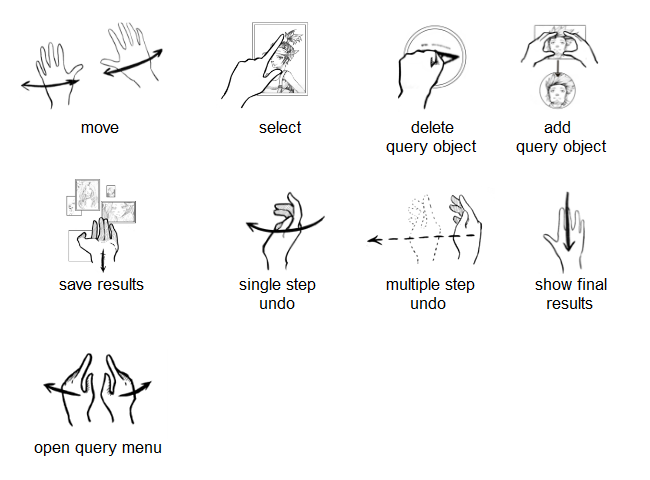
\includegraphics[width=1.8\marginparwidth]{figures/gestures.png}
  \caption{Gesten}
  \label{fig:gestures}
\end{figure}

\balance{} 


\bibliographystyle{SIGCHI-Reference-Format}
\bibliography{sample}

\end{document}

%%% Local Variables:
%%% mode: latex
%%% TeX-master: t
%%% End:
